\documentclass[journal]{new-aiaa}
\usepackage[utf8]{inputenc}
\usepackage{graphicx,amsmath,longtable,tabularx,booktabs,placeins}
\setlength\LTleft{0pt}
\graphicspath{{figures_revision/}}
\newcommand{\CM}{C_M^A}
\newcommand{\degc}{^\circ}
\title{Pre-Stall Load Redistribution on Swept Tailplane Models with Full-Span Controls}
\author{Andrea Rausa\footnote{PhD, Department of Aerospace Science and Technology, Corresponding Author, andrea.rausa@polimi.it},
Alex Zanotti\footnote{Associate Professor, Department of Aerospace Science and Technology}, Giuseppe Gibertini\footnote{Associate Professor, Department of Aerospace Science and Technology}, Alberto Guardone\footnote{Full Professor, Department of Aerospace Science and Technology}, and Franco Auteri\footnote{Full Professor, Department of Aerospace Science and Technology}}
\affil{Politecnico di Milano, Department of Aerospace Science and Technology, Milano, Italy, 20154}
\begin{document}
\maketitle
\begin{abstract}
Pre-stall changes in the integrated loads of swept lifting surfaces with full-span plain controls are examined using the existing MONNALISA wind-tunnel measurements and Reynolds-averaged Navier--Stokes solutions. The analysis distinguishes ordinary load increments from departures relative to empirical preceding trends and closes fixed-surface, control-surface, tip, and spatial budgets. For the positive-sweep, zero-dihedral model at a $20\degc$ control deflection, the fixed surface gains lift across the selected numerical interval but supplies about 63\% of the lift-growth deficit under the tested baseline and zero-incidence definitions. Both surface components contribute positively to the pitching-moment departure about the retained fitted aerodynamic center. Sectional pressures and complete spatial integrations show stronger ordinary leading-edge suction coexisting with reduced hinge-region loading and reduced growth of the fixed-surface contribution. Matched dihedral comparisons distinguish absolute load projection from incidence-dependent moment changes; the second planform also has reinforcing fitted-center moment departures. Experimental lift and moment features have separate sampled brackets and uncertainty limitations. Numerical correspondence is partial, including appreciable lift bias and missed or shifted features, so the detailed loading interpretation applies to the computed states. The contribution is the quantitative joint loading response and its spatial weighting, extending the previously published observation of control-surface separation.
\end{abstract}

\section*{Nomenclature}
\begin{longtable*}{@{}l@{\quad=\quad}l@{}}
$b$ & undeformed model semispan, m \\
$c,\ \bar c$ & local chord and mean aerodynamic chord (MAC), m \\
$C_L,C_D$ & lift and drag coefficients \\
$C_{F,x},C_{F,z}$ & body-axis force coefficients \\
$C_M^A$ & pitching-moment coefficient about the respective fitted center \\
$C_M^O,C_M^{A_I}$ & moment about numerical origin or common Geom.~I fitted axis \\
$C_p,\ \mathbf C_f$ & pressure and vector skin-friction coefficients \\
$D_{Q,j}$ & departure of component $j$ from its preceding coefficient trend \\
$f_{\mathrm{rev}}$ & specified upper-aft chordwise reversal area fraction \\
$m_{Q,j}^{\mathrm{pre}}$ & fitted preceding slope, per degree \\
$M_\infty,Re_{\bar c}$ & freestream Mach and MAC Reynolds numbers \\
$q_\infty,S$ & dynamic pressure and fixed semiplanform reference area \\
$s,\ \eta=s/b$ & undeformed span coordinate and its nondimensional value \\
$u_i$ & supplied propagated uncertainty magnitude at sample $i$ \\
$x_A,x_O$ & numerical fitted-center and original reference abscissae, m \\
$\alpha,\delta,\Gamma$ & displayed incidence, control deflection, and dihedral, deg \\
$\lambda,\Lambda,\tau$ & quarter-chord sweep, aspect ratio, and taper ratio \\
$\xi$ & local straightened chord fraction \\
BCM, SA & Bas--Cakmakcioglu transition and Spalart--Allmaras closure \\
RANS, WT & Reynolds-averaged Navier--Stokes and wind tunnel \\
\end{longtable*}

\section{Introduction}\label{sec:intro}
Separation and reduced effectiveness at large plain-flap deflections are established features of flapped lifting surfaces. The classical measurements of Sears and Liddell~\cite{sears1942plain} already documented reduced lift effectiveness associated with separation at large deflections. For swept finite wings, the distribution of loading and the progression of stall depend on planform and three-dimensional flow; sweep, aspect ratio, and taper cannot generally be treated as interchangeable variables~\cite{harper1964sweptstall}. Full-span plain controls are also established finite-wing configurations: Campbell, Blanks, and Leaver~\cite{campbell1956fullspan} measured lift, drag, and pitching moment on low-aspect-ratio rectangular wings with several flap chords. Neither the appearance of reversed flow over a highly deflected control nor continued growth of total lift after a local loss is, by itself, a new aerodynamic mechanism.

The question considered here is how local loading changes enter the integrated pre-stall response. A surface component can continue gaining lift while falling substantially below its preceding growth trend. An ordinary balance between increasing fixed-surface lift and decreasing control-surface lift therefore does not quantify the integrated nonlinearity. Pitching moment adds a second distinction: similar lift changes at different chordwise or spanwise locations have different moment weights. A useful analysis must quantify these contributions with consistent normalization, incidence samples, and moment references.

The MONNALISA database publication~\cite{rausa2026monnalisa} provides the measurements and saved numerical solutions used here. Its Sec.~IV and Fig.~11 already describe the baseline pre-stall lift nonlinearity, expanding reversed flow on the control, pressure changes, and continued growth of total lift. It also reports nonlinear lower-fidelity behavior. The present work extends that material through additive ordinary-increment and preceding-trend-departure budgets, complete spatial load changes, quantitative reversal measures, separately characterized experimental moment features, and matched control-deflection comparisons between the two available dihedral settings. The source dataset and baseline separation observation are reused explicitly.

These are isolated tailplane-inspired wing models, without a fuselage, wing wake, or complete-aircraft trim condition. Full-span control extent and a 30\%-chord control are the tested geometry choices. Partial-span controls and other flap chords are outside the dataset; no cutoff in spanwise extent is inferred. The $45\degc$ dihedral setting provides a large controlled change in orientation on the same planform, rather than a representative value for conventional horizontal tails. A second planform provides a separate comparison in which several geometric parameters change together.

Lower computational order does not imply a necessarily linear response. Nonlinear lifting-line methods can incorporate sectional viscous data~\cite{sivells1947liftingline}. In MONNALISA, the DUST lifting-line formulation uses sectional tables and corrections, whereas the retained potential-based panel and vortex-lattice predictions are smoother~\cite{rausa2026monnalisa}. This model-specific evidence precludes a general claim that low-order methods cannot capture pre-stall nonlinear signatures. Here, the detailed surface accounting is drawn from RANS, and its correspondence with the measured integrated coefficients is assessed before interpreting the numerical loading changes.

\section{Experimental, Numerical, and Analysis Framework}\label{sec:methods}
\subsection{Models and experimental installation}\label{sec:setup}
The models have an undeformed semispan $b=1.6$~m, nominal thickness ratio $t/c=9\%$, and a full-span plain trailing-edge control rotating about the 70\%-chord hinge. Table~\ref{tab:geometry} gives the geometry and global references. Aspect ratio is defined for the corresponding full planform, $\Lambda=2b^2/S$. Geom.~I at $\Gamma=0\degc$ and $45\degc$ retains the same undeformed planform, area, and MAC. Geom.~II simultaneously changes sweep, taper, aspect ratio, area, and chord distribution. It is a planform comparison, rather than an isolated sweep-direction test.

\begin{table}[htbp]\centering
\caption{Geometry and reference quantities. Area is the undeformed semiplanform area; $Re_{\bar c}=Re_b\bar c/b$, with $Re_b=5.5\times10^6$.}\label{tab:geometry}
\begin{tabular}{lccc}\toprule
Property & I, $\Gamma=0\degc$ & I, $\Gamma=45\degc$ & II, $\Gamma=0\degc$ \\\midrule
$\lambda$ (deg) & 30 & 30 & $-15$ \\
$\Lambda$ & 5.0 & 5.0 & 5.2 \\
$\tau$ & 0.4 & 0.4 & 0.6 \\
$S$ (m$^2$) & 1.024 & 1.024 & 0.984604 \\
$\bar c$ (m) & 0.679184 & 0.679184 & 0.6282 \\
Root chord (m, rounded) & 0.914286 & 0.914286 & 0.76923 \\
$Re_{\bar c}$ & $2.335\times10^6$ & $2.335\times10^6$ & $2.159\times10^6$ \\
Numerical $x_A$ (m) & 0.642000 & 0.643532 & $-0.003618$ \\\bottomrule
\end{tabular}
\end{table}

\begin{figure}[htbp]\centering
\begin{minipage}[c]{.28\textwidth}\centering
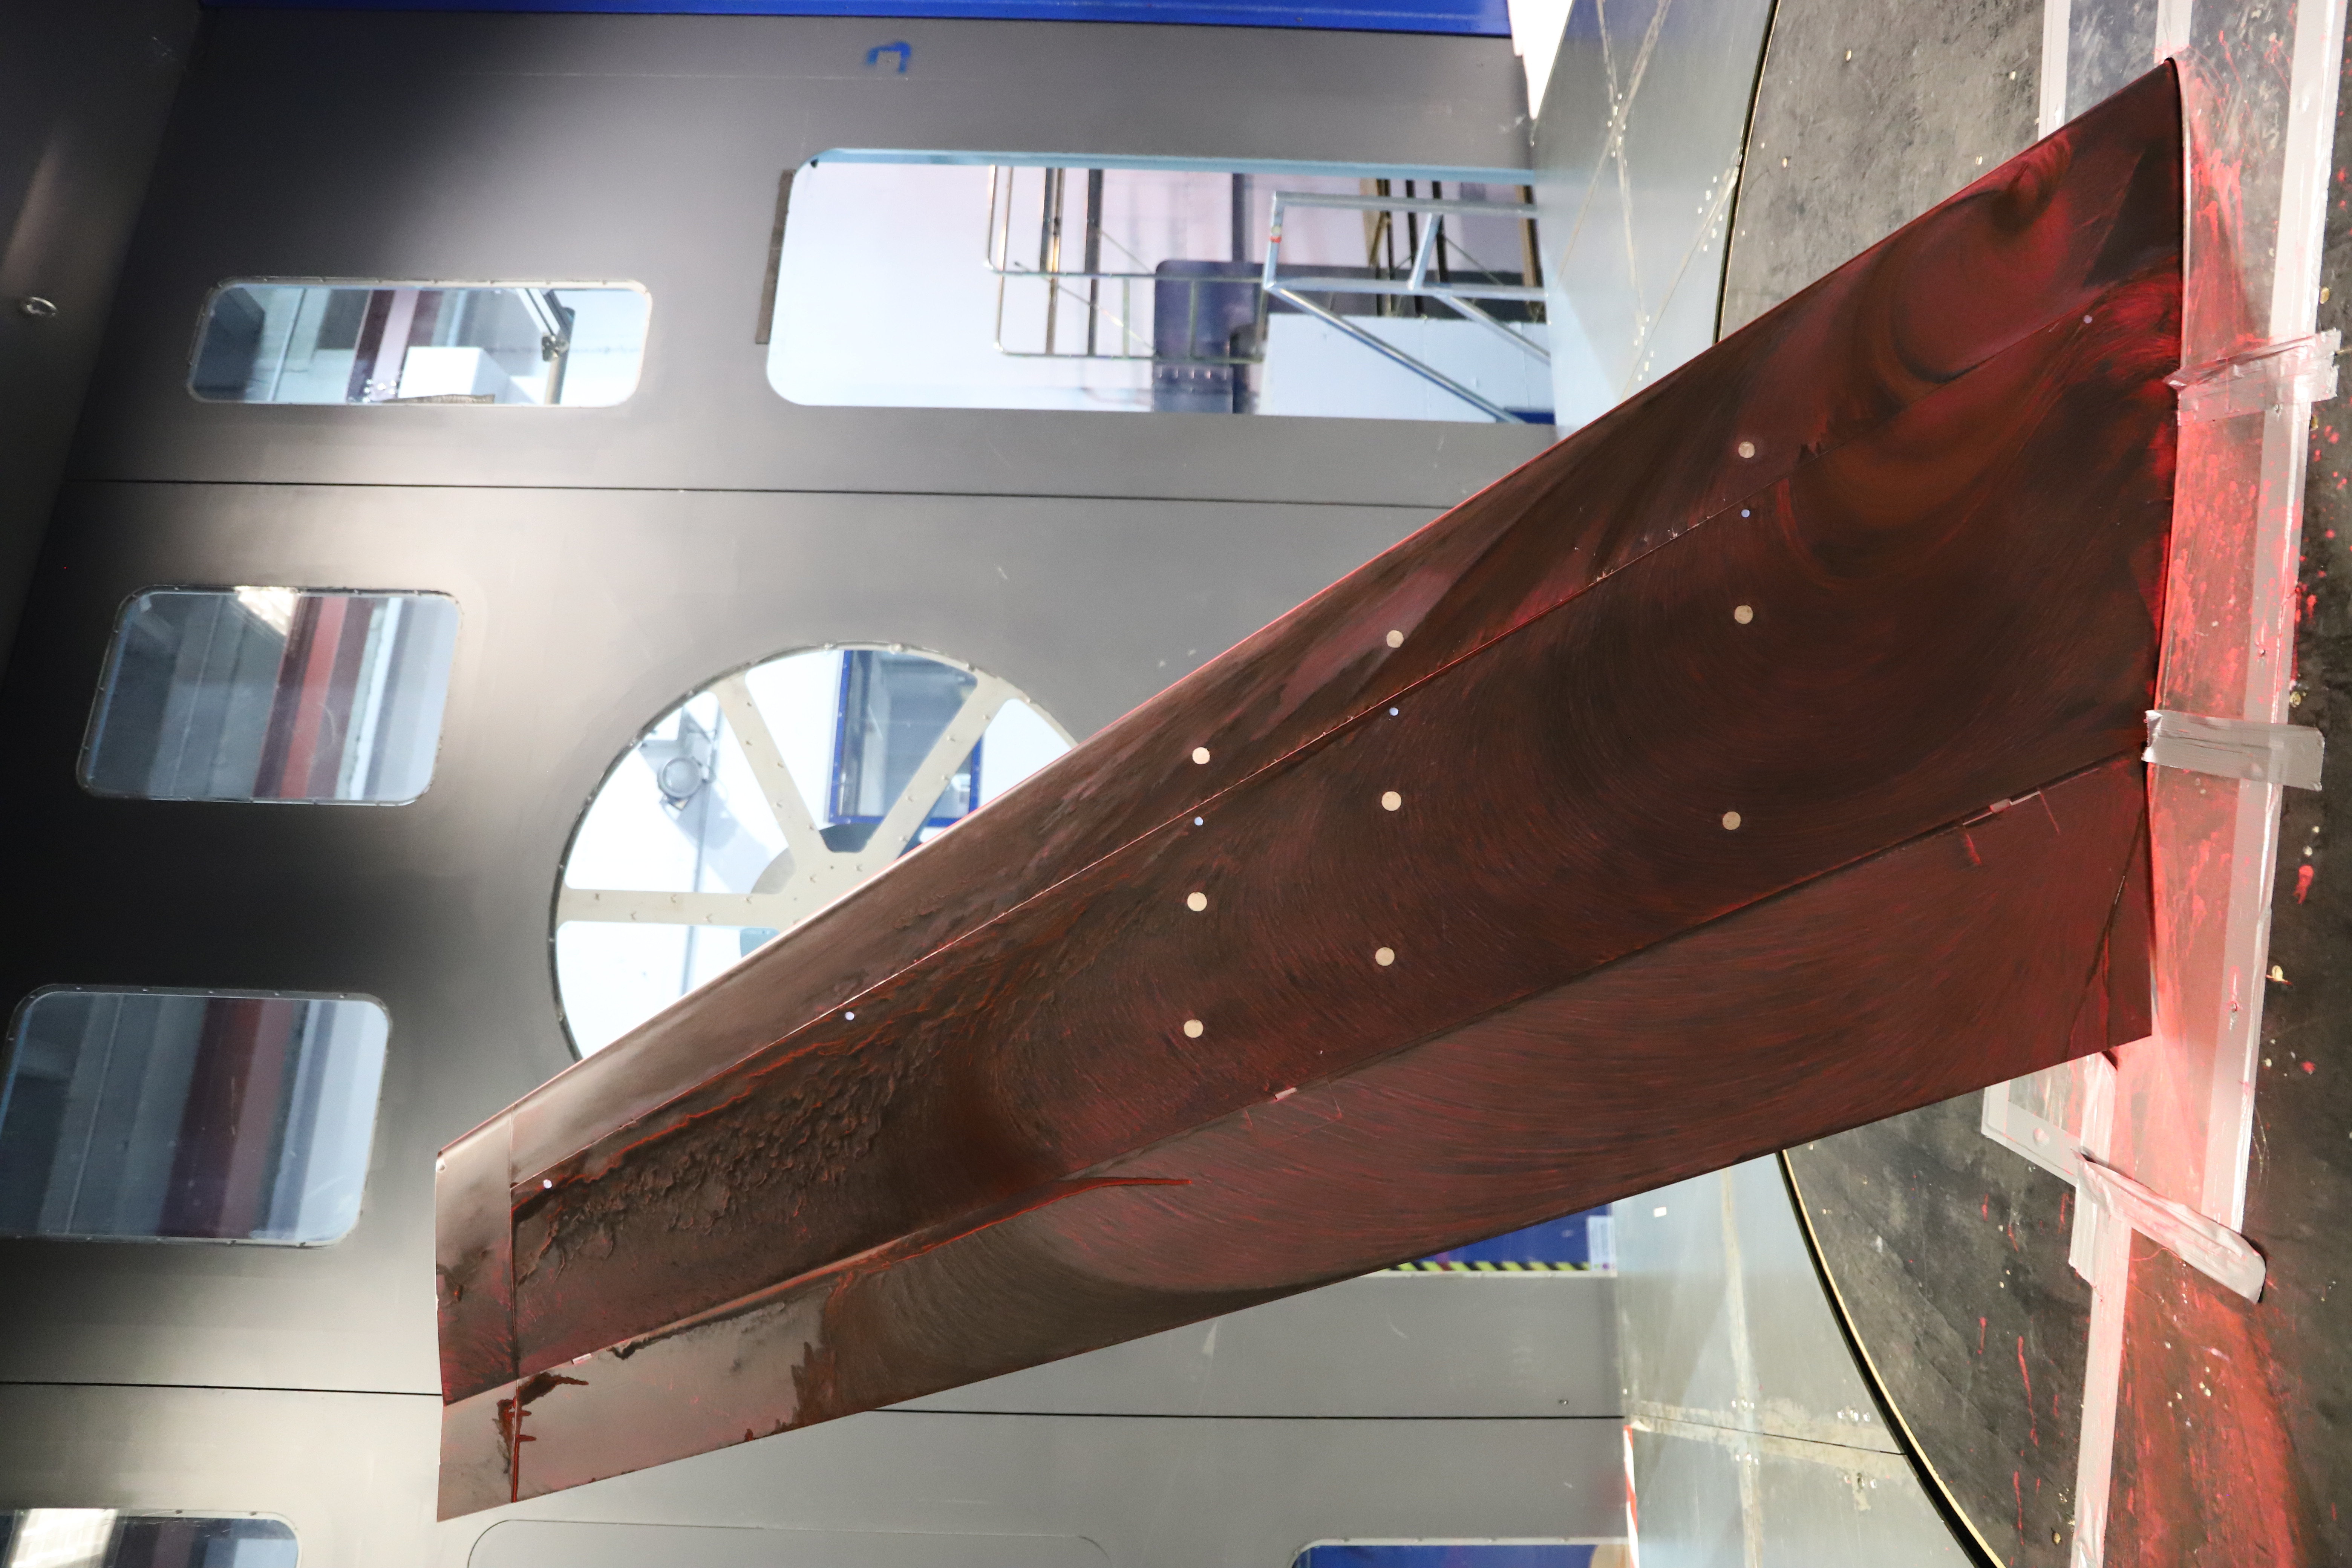
\includegraphics[angle=-90,origin=c,width=\linewidth]{installation.JPG}\\(a)
\end{minipage}\hfill
\begin{minipage}[c]{.70\textwidth}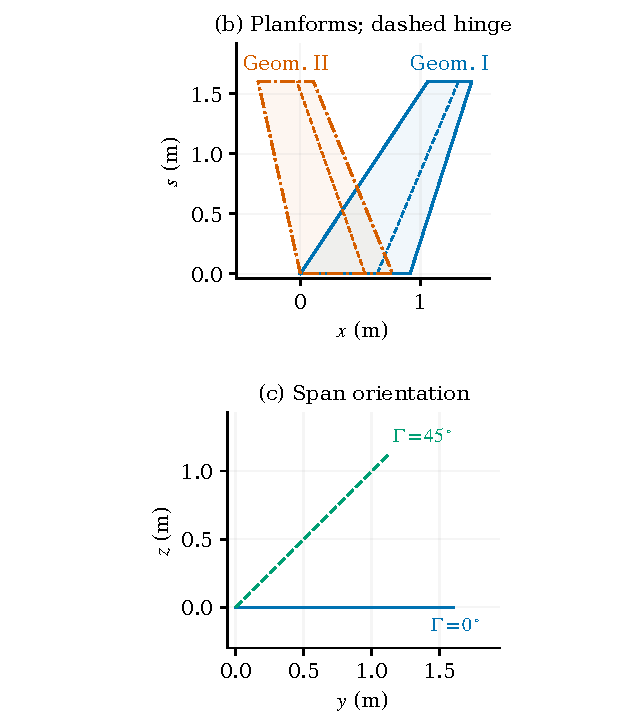
\includegraphics[width=\linewidth]{geometry.pdf}\end{minipage}
\caption{Model installation and geometries: (a) archived oil-flow photograph in the GVPM installation, recorded in the $\alpha=25\degc$, $\delta=20\degc$ test folder, used only to illustrate mounting; (b) undeformed planforms and 70\%-chord hinges; (c) numerical span orientation at the two dihedral settings. The photograph is not evidence of the pre-stall flow state. The planform dimensions are in Table~\ref{tab:geometry}.}\label{fig:setup}
\end{figure}

The WT measurements were obtained in the low-turbulence section of the closed-circuit GVPM facility at Politecnico di Milano. Figure~\ref{fig:setup} shows the floor-mounted semispan installation. The dummy floor conceals the support, balance, and control actuation mechanism. The documented test-section width and length are 4 and 6~m, respectively; the undeformed semispan is 40\% of that width. A consistent installed-height value and a floor-layer profile at the model are unavailable for a quantitative confinement assessment. Thus neither a thin floor layer nor negligible wall effects is assumed.

The database setup description~\cite{rausa2026monnalisa} gives freestream turbulence below 0.1\%, measured using a turbulence sphere and hot-wire anemometry. Outside the wall layers, the inlet total-pressure variation was within $\pm0.5\%$ of dynamic pressure over most of the section and within $\pm1\%$ overall; outlet measurements confirmed similar uniformity. The reported longitudinal static-pressure gradient is $\partial C_P/\partial x=-0.004$~m$^{-1}$. Loads were acquired through a RUAG 767 strain-gauge balance below the floor and an HBM QuantumX system; the reduction includes the balance-to-wind transformation and the database corrections. Nominal conditions are $M_\infty=0.147$, $T_\infty=300$~K, and the MAC Reynolds numbers in Table~\ref{tab:geometry}. The span-based database Reynolds number is retained only for traceability.

Only the author's LE1 experimental profile variant is used. Its recorded incidences are $-25,-24,-22,\ldots,22,24,25\degc$: the local pre-stall spacing is $2\degc$, with $1\degc$ endpoint steps. The present comparison uses $\delta=0,10,20,30\degc$; the database also contains other deflections. The uncertainty bars are the supplied propagated measurement/reduction-chain magnitudes, including balance and transformation contributions. For the fitted-center moment, its supplied central value and associated propagated uncertainty are kept paired. They are not replaced by repeat-run scatter. No common coverage factor is assigned here, and between-incidence covariance is unavailable. Numerical uncertainty sensitivities of experimental contrasts are defined separately below.

\subsection{Conventions and moment references}\label{sec:references}
In the numerical body axes, $x$ is downstream, $y$ is spanwise, and $z$ is upward. The force rotation and normalization are
\begin{equation}
 C_L=C_{F,z}\cos\alpha-C_{F,x}\sin\alpha,\qquad
 C_D=C_{F,z}\sin\alpha+C_{F,x}\cos\alpha,\qquad
 C_{F,k}=F_k/(q_\infty S).
\label{eq:force}
\end{equation}
Pitching moment is positive nose-up and normalized by $q_\infty S\bar c$. Table~\ref{tab:mapping} summarizes the retained angle and frame mapping. No further angle flip or alignment shift is applied to improve agreement.

\begin{table}[htbp]\centering
\caption{Conversion to the displayed convention. Subscript $r$ denotes the existing reduced WT record; $n$ denotes a native numerical state.}\label{tab:mapping}
\begin{tabularx}{\textwidth}{lX}\toprule
Source & Displayed quantities and state handling \\\midrule
Reduced WT & $\alpha=-\alpha_r$, $\delta=\delta_r$, $C_L=-C_{L,r}$, $\CM=-C_{M,r}^{A}$; drag and uncertainty magnitudes retain their signs. \\
RANS, direct & Native $\alpha_n,\delta_n$ retained; forces use Eq.~\ref{eq:force}. \\
RANS, $\Gamma=0\degc$ reflected & Opposite-deflection parent gives $\alpha=-\alpha_n$, $\delta=-\delta_n$. Positions/forces transform with $T=\mathrm{diag}(1,1,-1)$; moments with $(\det T)T$; physical sides exchange. \\
RANS, $\Gamma=45\degc$ & Signed incidence is directly computed; no same-dihedral reflection. \\
Zero incidence & Direct and reflected opposite-deflection parents remain distinct. Each interpreted field uses its own saved force state. \\\bottomrule
\end{tabularx}
\end{table}

The principal WT--RANS comparison retains the moments about the respective zero-deflection fitted aerodynamic centers, denoted $\CM$. Following the database construction~\cite{rausa2026monnalisa}, the reference is obtained from linear fits to zero-deflection moment and force over $|\alpha|\leq10\degc$ and then held fixed for all control deflections. The WT reduction uses uncertainty-weighted fits; the retained numerical references use their historical linear fits. This compares the same reference construction across datasets, rather than identical physical axes. It is neither an instantaneous aerodynamic center nor necessarily quarter-MAC. The WT moment is not transported onto a numerical axis without a physical registration.

The original numerical reference is $O=(0.228571,0,0)$~m, the root quarter-chord of Geom.~I. For a numerical pole displaced only in $x$,
\begin{equation}
 C_M(x_1)=C_M(x_0)+\frac{x_1-x_0}{\bar c}C_{F,z}.
\label{eq:transport}
\end{equation}
The fitted abscissae are in Table~\ref{tab:geometry}. Matched dihedral diagnostics use the identical numerical axis $A_I=(0.642000,0,0)$~m in both configurations, denoted $C_M^{A_I}$. Geom.~II uses its own MAC once for every moment contribution; all coefficients use the fixed areas in Table~\ref{tab:geometry}.

\subsection{Numerical method and existing accuracy evidence}\label{sec:numerics}
The existing SU2~\cite{palacios2013stanford} solutions use compressible ideal-gas RANS at the nominal WT Mach and Reynolds conditions, with Sutherland viscosity. Unstructured finite volumes use median-dual vertex control volumes. Mean-flow convection uses Roe fluxes with second-order MUSCL reconstruction~\cite{van1979towards}, Green--Gauss gradients, and a Venkatakrishnan limiter~\cite{venkatakrishnan1993accuracy} with coefficient 0.05. SA~\cite{spalart1992sa} convection uses scalar upwinding without MUSCL, hence first-order reconstruction. The BCM transition closure~\cite{cakmakcioglu2020bcm} supplies an algebraic intermittency correction, not an independently transported transition equation. Spatial order must therefore be distinguished between mean-flow and SA equations.

The surfaces have no-slip, zero-heat-flux boundaries; the exterior uses a far-field boundary and the root plane a symmetry boundary. This excludes the WT floor, its layer, and the support. Implicit Euler pseudo-time advancement, FGMRES linear solves, adaptive CFL, and staged restarts were used to obtain steady states. The configured Cauchy stopping criterion monitors lift and drag over 100 entries, commonly at $3\times10^{-6}$ and at $10^{-6}$ in later Geom.~II stages. Moment is not a stopping quantity; iteration caps and restarts also occur.

Saved terminal histories match the force reports for 41 of the 44 selected surface states. Three lack such a terminal match: Geom.~I/$\Gamma=0\degc$, displayed $\alpha=-6\degc$, $\delta=30\degc$; and Geom.~II/$\delta=20\degc$, displayed $\alpha=-4\degc$ and direct $0\degc$. This is incomplete iterative registration, not proof of failed solves. For the dihedral $\delta=20\degc$ irregularity between $-6$ and $-4\degc$, the matching histories' last-100 lift ranges are approximately $10^{-4}$, much smaller than the between-state change. Not every saved state has a complete final-stage reconstruction-order registration. Saved-state consistency does not establish global steady-flow uniqueness or physical accuracy.

The automated mesh procedure~\cite{rausa2026monnalisa} uses anisotropic surface triangles, leading-edge and hinge/junction refinement, a hex-dominant octree volume, and incidence-oriented wake refinement. Nominal controls are a $2.5\degc$ leading-edge angle, $1\degc$ junction angle, seven trailing-edge points, maximum surface spacing 0.02~m, and boundary-layer growth ratio 1.15. Actual first-cell height and layer count are not registered for every retained mesh. Representative stored $y^+$ medians are 0.26 for I/$\delta=20\degc$/$\alpha=2\degc$, 0.19 for I/$\Gamma=45\degc$/$\delta=30\degc$/$\alpha=0\degc$, and 0.23 for II/$\delta=20\degc$/$\alpha=0\degc$, with maxima approximately 1.22, 1.26, and 1.13. These support resolved near-wall treatment for those samples.

Selected surface meshes have 122,860 points/182,423 elements for I/$\delta=20\degc$ at $0,2,4\degc$, 141,828/209,641 for I/$\Gamma=45\degc$/$\delta=30\degc$ at $-2,0,2\degc$, and 105,506/156,333 for II/$\delta=20\degc$ at $0,2,4\degc$. These are surface counts. The retained volume for the I/$\alpha=0\degc$/$\delta=-20\degc$ parent contains 9,440,030 points and 18,918,212 volume elements; equivalent registered volume counts are not available for every interpreted state.

Table~\ref{tab:mesh} brings the existing four-level mesh study into the present article. It concerns Geom.~I at $\delta=35\degc$, $\Gamma=0,45\degc$, and $\alpha=0,18\degc$. The published lift/drag assessment is augmented only by moments linked to the same retained states. Nominal-to-finest differences are 1.20--2.14\% for lift and 1.13--2.49\% for drag. The moment gap at $\Gamma=0\degc$, $\alpha=18\degc$ is 0.01343; the inclined sequence is nonmonotonic. This is inherited integrated-load sensitivity evidence, without an asymptotic-order or discretization-uncertainty estimate. It does not establish convergence of the current $20/30\degc$ departures, regional loads, pressure sections, or separation topology, nor of Geom.~II.

\begin{table}[htbp]\centering\small
\caption{Existing four-level Geom.~I study, $\delta=35\degc$. Grid counts are in millions. $C_M^O$ uses $O=(0.228571428571,0,0)$~m and the Geom.~I area/MAC. Missing finest $\alpha=0\degc$ moments have no matching saved force/history state and are not assigned to the historical lift/drag rows.}\label{tab:mesh}
\begin{tabular}{rrlrrrrr}\toprule
$\Gamma$ & $\alpha$ & Level & Points & Volume elements & $C_L$ & $C_D$ & $C_M^O$ \\\midrule
0 & 0 & Coarse & 4.791 & 9.513 & 0.814498 & 0.119412 & -0.673479 \\
0 & 0 & Nominal & 9.942 & 19.966 & 0.812040 & 0.119153 & -0.671422 \\
0 & 0 & Fine & 22.555 & 40.514 & 0.825137 & 0.117927 & -0.678262 \\
0 & 0 & Very fine & 50.113 & 87.354 & 0.829782 & 0.116264 & -- \\
45 & 0 & Coarse & 5.130 & 10.520 & 0.601545 & 0.135739 & -0.409031 \\
45 & 0 & Nominal & 9.672 & 19.065 & 0.595119 & 0.134514 & -0.405495 \\
45 & 0 & Fine & 22.331 & 39.928 & 0.576407 & 0.136639 & -0.394208 \\
45 & 0 & Very fine & 51.800 & 91.679 & 0.588083 & 0.136059 & -- \\
0 & 18 & Coarse & 4.853 & 9.627 & 1.003433 & 0.469819 & -0.801593 \\
0 & 18 & Nominal & 12.738 & 24.066 & 1.014062 & 0.478558 & -0.813372 \\
0 & 18 & Fine & 26.555 & 45.699 & 1.020499 & 0.484723 & -0.819923 \\
0 & 18 & Very fine & 65.241 & 105.956 & 1.026778 & 0.488463 & -0.826802 \\
45 & 18 & Coarse & 5.291 & 10.904 & 0.646962 & 0.328149 & -0.407668 \\
45 & 18 & Nominal & 9.966 & 19.455 & 0.642268 & 0.332710 & -0.407173 \\
45 & 18 & Fine & 25.140 & 43.937 & 0.632794 & 0.338850 & -0.405896 \\
45 & 18 & Very fine & 65.894 & 109.982 & 0.633456 & 0.341097 & -0.407091 \\

\bottomrule\end{tabular}
\end{table}

\subsection{Additive loading and empirical departures}\label{sec:analysis}
Solver surface groups define the fixed surface (upper/lower fixed panels), the control (upper/lower control panels, hinge junction, and blunt trailing edge), and tip. Pressure and viscous contributions are retained on both physical sides with the same global $S$ and $\bar c$. Tip is included in every total; no component is multiplied for display.

For coefficient $Q$ and component $j$, define
\begin{equation}
 \Delta C_{Q,j}=C_{Q,j}(\alpha_b)-C_{Q,j}(\alpha_a),\qquad
 D_{Q,j}=\Delta C_{Q,j}-m_{Q,j}^{\mathrm{pre}}(\alpha_b-\alpha_a).
\label{eq:departure}
\end{equation}
The preceding slope is an unweighted linear least-squares fit to the declared actual samples. All additive components and the total use identical samples and weights, preserving their sum. The primary $\delta=20\degc$ baseline is $\{-6,-4,-2\}\degc$; the early I/$\delta=30\degc$ numerical baseline is $\{-16,-14,-12\}\degc$. Each is an empirical reference, without an assumption that the preceding flow is attached. Adjacent windows and both zero parents test sensitivity. Curved sequences are described using signed finite differences rather than a forced unique event amplitude.

For WT contrasts, Eq.~\ref{eq:departure} is written as $D=\sum_i w_iC_i$, combining repeated uses of any sample into one weight. The two reported sensitivities are
\begin{equation}
 u_{\mathrm{ind}}=\left[\sum_i(w_i u_i)^2\right]^{1/2},\qquad
 u_{\mathrm{L1}}=\sum_i|w_i|u_i.
\label{eq:uncertainty}
\end{equation}
The first is conditional on independence; the second bounds a perturbation when each sample varies within its supplied magnitude. Neither is an established confidence interval or a new experimental uncertainty budget. Covariance-dependent significance is not inferred.

Saved nodal $C_p$ and vector $\mathbf C_f$ are integrated over the complete triangulated surface. Linear traction and position-times-traction are integrated exactly within each triangle, with
\begin{equation}
 C_M(x_A)=\frac{1}{q_\infty S\bar c}
 \int\big[z\,dF_x-(x-x_A)dF_z\big].
\label{eq:moment}
\end{equation}
The two terms are retained separately where a common-axis dihedral comparison needs them. All 44 full-surface reconstructions have endpoint residuals below $1.5\times10^{-4}$. Maximum lift and moment residuals are $2.71\times10^{-5}$ and $7.06\times10^{-5}$. Conservative absolute-weight residual bounds are checked separately against each increment or departure, with a 10\% effect-scale limit for an adopted interpretation. For the baseline lift departure, the bound is $1.01\times10^{-5}$ against $|D_L|=0.11060$. Small shear changes that fail their corresponding bound are not assigned a resolved mechanism. Accounting closure and reconstruction agreement are distinct from iteration, mesh sensitivity, and experiment--model discrepancy; global residuals do not bound each regional error.

Geometric bins use $\eta=s/b$ and straightened $\xi$, obtained by undoing the control rotation about the three-dimensional hinge. They include both sides and root extensions; end faces are retained separately. Whole triangles are assigned by centroid. These bins differ from native solver markers, especially at the hinge junction. Sectional pressure curves use $\eta=0.2,0.5,0.8$ and preserve actual contour connectivity on the native upper/lower fixed and control panels, excluding junction and end faces. Three sections illustrate pressure changes; complete integrations supply the budgets.

A chordwise reversal indicator measures the actual upper geometric-aft area ($\xi\geq0.7$, excluding end caps) on which $\mathbf C_f\cdot\mathbf t_c<-\epsilon$, with downstream chord direction projected into the face tangent. Linear nodal signs are clipped within triangles. The fraction $f_{\mathrm{rev}}$ is tested at $\epsilon=0,10^{-6},10^{-5}$. It measures a specified component of reversed shear, rather than the full three-dimensional separation footprint.
\FloatBarrier

\section{Measured Response and Numerical Correspondence}\label{sec:response}
Figure~\ref{fig:measured} presents the baseline measured loads, including $\delta=10\degc$ as a lower-deflection control. Figure~\ref{fig:comparison} combines the principal WT--RANS comparisons at the respective fitted references. Horizontal brackets mark sampled experimental changes; they are not continuously determined onset angles. Table~\ref{tab:wt} quantifies selected preceding-trend contrasts with the supplied uncertainty sensitivities.

\begin{figure}[htbp]\centering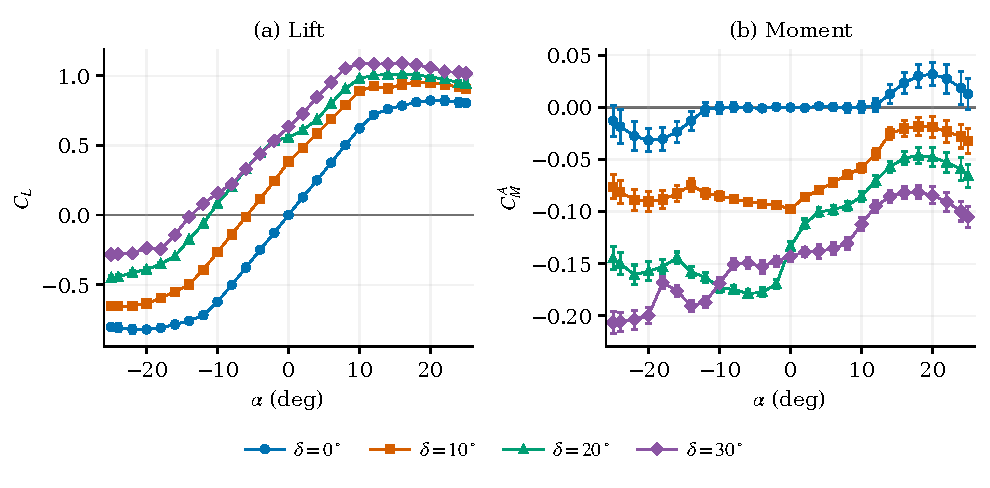
\includegraphics[width=\textwidth]{measured_baseline.pdf}
\caption{LE1 WT response of Geom.~I, $\Gamma=0\degc$, for $\delta=0,10,20,30\degc$. Moment $C_M^A$ uses the experimental zero-deflection fitted center, held fixed across deflection. Bars are the paired supplied propagated magnitudes, without an assigned common coverage factor.}\label{fig:measured}\end{figure}

\begin{figure}[htbp]\centering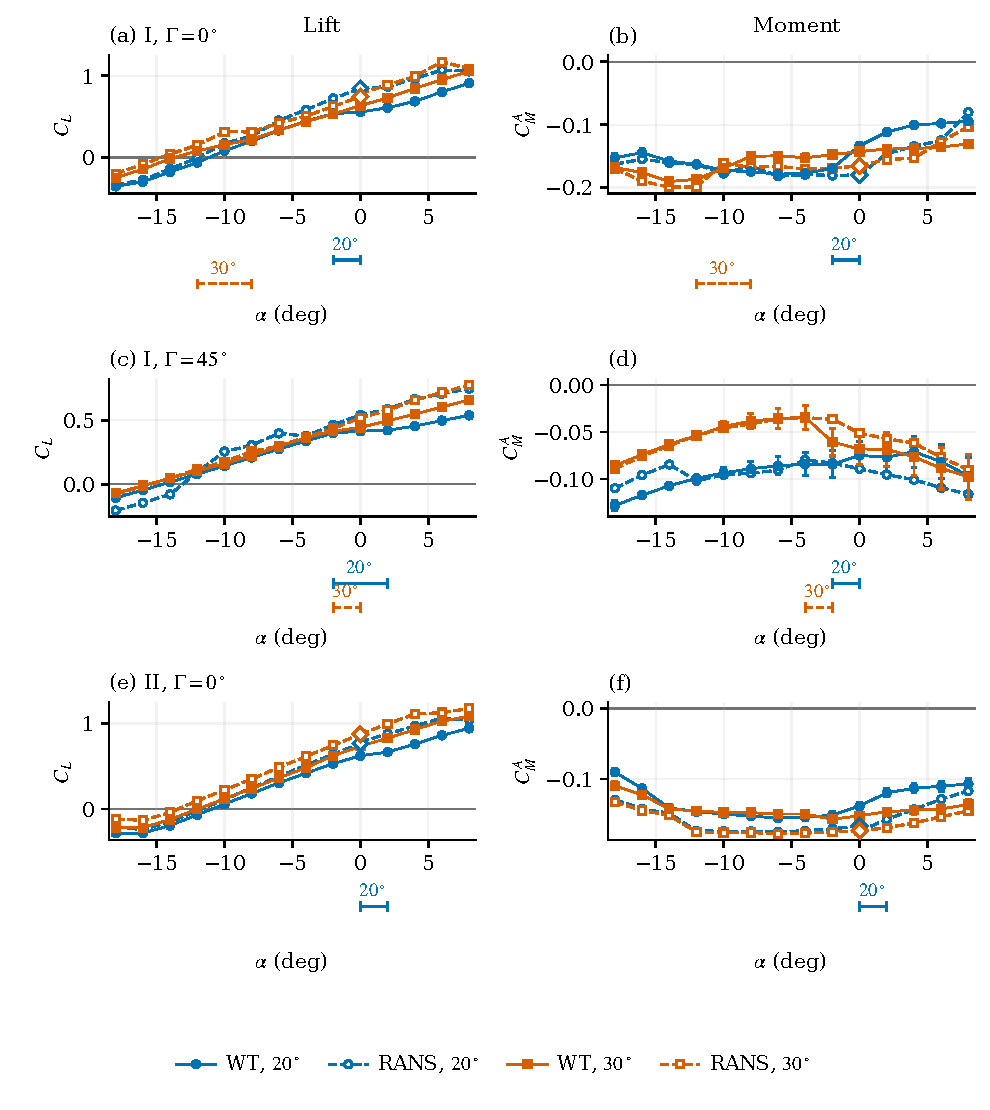
\includegraphics[width=.96\textwidth]{comparison.pdf}
\caption{Measured and computed pre-stall loads: Geom.~I at $\Gamma=0\degc$ (a,b) and $45\degc$ (c,d), and Geom.~II at $\Gamma=0\degc$ (e,f). Filled symbols/solid lines: LE1 WT; open symbols/dashed lines: RANS. Circles and squares distinguish $\delta=20\degc$ and $30\degc$. Horizontal brackets labeled by deflection show the selected WT incidence intervals. Moment uses each dataset's own zero-deflection fitted center. Open diamonds at zero incidence distinguish reflected opposite-deflection parents, without averaging or curve shifts.}\label{fig:comparison}\end{figure}

\begin{table}[htbp]\centering\small
\caption{Primary LE1 WT departure contrasts. Each baseline is $\{-6,-4,-2\}\degc$; brackets are selected separately for lift and moment. Moment uses the WT fitted center. $u_{\mathrm{ind}}$ and $u_{\mathrm{L1}}$ are the full-contrast sensitivities of Eq.~\ref{eq:uncertainty}, not confidence limits.}\label{tab:wt}
\begin{tabular}{llrrrr}\toprule
Geom., $\Gamma$, $\delta$ & Coefficient & Interval (deg) & $D$ & $u_{\mathrm{ind}}$ & $u_{\mathrm{L1}}$ \\\midrule
I, $0^\circ$, $20^\circ$ & $C_L$ & $-2\to0$ & -0.08274 & 0.02357 & 0.03631 \\
I, $0^\circ$, $20^\circ$ & $C_M^A$ & $-2\to0$ & +0.03148 & 0.00862 & 0.01360 \\
I, $45^\circ$, $20^\circ$ & $C_L$ & $-2\to0$ & -0.04785 & 0.01694 & 0.02634 \\
I, $45^\circ$, $20^\circ$ & $C_M^A$ & $-2\to0$ & +0.00847 & 0.02630 & 0.04082 \\
I, $45^\circ$, $30^\circ$ & $C_L$ & $-2\to0$ & -0.04038 & 0.01646 & 0.02996 \\
I, $45^\circ$, $30^\circ$ & $C_M^A$ & $-4\to-2$ & -0.02860 & 0.02478 & 0.03822 \\
II, $0^\circ$, $20^\circ$ & $C_L$ & $0\to2$ & -0.06902 & 0.02090 & 0.03739 \\
II, $0^\circ$, $20^\circ$ & $C_M^A$ & $0\to2$ & +0.01668 & 0.00793 & 0.01424 \\

\bottomrule\end{tabular}\end{table}

For I/$\Gamma=0\degc$/$\delta=20\degc$, measured lift grows by only 0.01987 over $-2\to0\degc$, compared with 0.08922 over $-4\to-2\degc$. The primary departure is $-0.08274$, exceeding both stated sensitivities. Across the selected bracket, pointwise lift uncertainty magnitudes are approximately 0.01271--0.01328. Moment increases by $+0.03605$: the negative coefficient becomes less negative, rather than crossing zero. Its primary departure is $+0.03148$, versus $u_{\mathrm{L1}}=0.01360$, and pointwise moment magnitudes are approximately 0.00461--0.00468. These signed changes are established at the sampled resolution; they do not locate a sharp discontinuity or uniquely identify a local topology.

At $\delta=30\degc$, the measured early lift increments are $+0.07654$, $+0.06419$, and $+0.11131$ over $-12\to-10$, $-10\to-8$, and $-8\to-6\degc$. Moment already increases by $+0.01800$ and $+0.01828$ on the first two intervals. Its relevant early change cannot be assigned only to incidence near $-2\degc$. The preceding lift sequence is curved: adjacent empirical windows yield departures of both signs, approximately $-0.03971$ to $+0.02865$. Actual interval slopes provide the more reliable description of this broad feature. At $\delta=10\degc$, the moment increment changes from $-0.00384$ over $-2\to0\degc$ to $+0.01126$ over $0\to2\degc$. Thus a universal $20\degc$ threshold for joint lift/moment nonlinearity is unsupported.

For I/$\Gamma=45\degc$/$\delta=20\degc$, measured lift growth remains suppressed across $-2\to2\degc$: successive increments are $+0.01475$ and $+0.00748$. The positive moment increment over $-2\to0\degc$ is $+0.00934$, but its departure is smaller than both uncertainty sensitivities (Table~\ref{tab:wt}). Absence of a resolved moment feature is therefore not evidence of absent redistribution. At $\delta=30\degc$, the strongest selected lift slowdown is $-2\to0\degc$; the moment decreases algebraically by $-0.02649$ earlier, over $-4\to-2\degc$. Its departure is comparable with $u_{\mathrm{ind}}$ and smaller than $u_{\mathrm{L1}}$. These are different, uncertainty-qualified coefficient brackets.

For II/$\delta=20\degc$, measured lift grows by $+0.04403$ over $0\to2\degc$, compared with $+0.09214$ before and $+0.09204$ after. Moment increases by $+0.01872$. The primary moment departure exceeds the reported sensitivities, although adjacent-window departures range from $+0.01074$ to $+0.01956$ and do not uniformly exceed the primary L1 magnitude. The larger-deflection comparison is retained in Fig.~\ref{fig:comparison}; it does not establish a common abrupt event for every deflection.

Numerical correspondence must be assessed separately for each coefficient. The baseline I/$\delta=20\degc$ RANS lift slowdown occurs over $0\to2\degc$, one sampled interval later than the measured bracket. At zero incidence its two retained lift states are approximately 0.84217 and 0.84335, versus WT 0.55596 with supplied magnitude 0.01328. This appreciable bias accompanies a qualitatively similar slowdown and a less-negative moment response; no alignment shift is used. The early I/$\delta=30\degc$ numerical lift change is also sharper than the broad experimental change, and its fitted-center moment departure is window-sensitive.

At $\Gamma=45\degc$, numerical $\delta=20\degc$ lift decreases from 0.39722 at $-6\degc$ to 0.37618 at $-4\degc$, whereas WT increases by 0.06324. The numerical sequence does not convincingly reproduce the measured sustained slowdown or its weak moment response. At $\delta=30\degc$, a negative moment change is qualitatively present, but its strongest numerical bracket is later than the measured $-4\to-2\degc$ interval. For II/$\delta=20\degc$, the direct numerical $0\to2\degc$ lift increment is $+0.09351$, more than twice the measured $+0.04403$: the measured slowdown is not reproduced convincingly in amplitude. The corresponding fitted-center moment increment, $+0.01682$, is locally close to $+0.01872$, with the distinct reference constructions retained.

Consequently, the following pressure, reversal, and component analyses explain the computed load response. Nominally corresponding WT conditions do not experimentally validate these detailed topologies. The symmetry-root/floor difference is a scope limitation; the present comparisons do not attribute the residuals to floor or tunnel effects.
\FloatBarrier

\section{Joint Numerical Loading Response}\label{sec:joint}
\subsection{Ordinary growth and reduced growth of the fixed surface}\label{sec:budget}
Figure~\ref{fig:budget} and Table~\ref{tab:budget} give the central numerical budget. For I/$\Gamma=0\degc$/$\delta=20\degc$ over the direct $0\to2\degc$ interval, fixed-surface lift increases by $+0.05929$ while control lift decreases by $-0.03510$. Their ordinary balance yields a small positive total increment, $+0.02418$. Relative to the shared baseline $\{-6,-4,-2\}\degc$, however, both components fall below their preceding trends: $D_{L,\mathrm{fixed}}=-0.06918$ and $D_{L,\mathrm{control}}=-0.04143$, with total $D_L=-0.11060$. Positive ordinary fixed-surface growth is therefore compatible with a substantial fixed-surface contribution to the lift nonlinearity.

\begin{figure}[htbp]\centering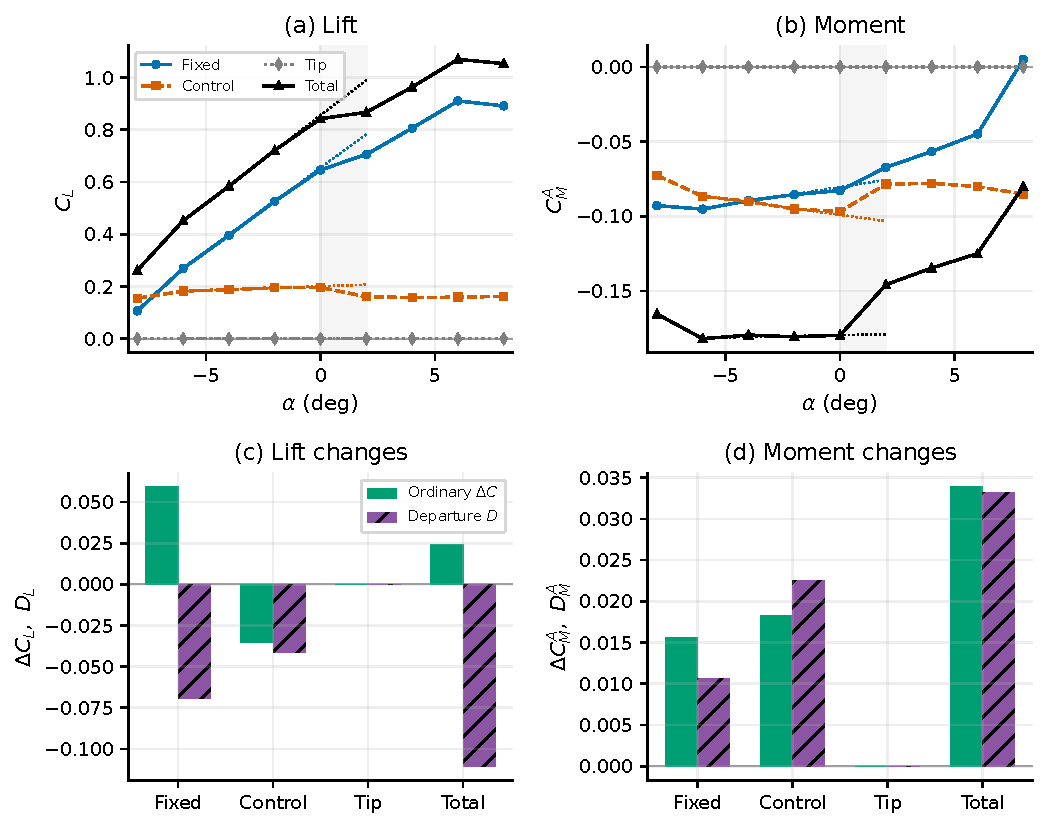
\includegraphics[width=\textwidth]{baseline_budget.pdf}
\caption{Geom.~I, $\Gamma=0\degc$, $\delta=20\degc$: fixed, control, tip, and total numerical coefficients and changes. Moment uses the retained I/$\Gamma=0\degc$ fitted axis $x_A=0.642000000830$~m. Dotted lines extrapolate unweighted fits to $\{-6,-4,-2\}\degc$. The shaded $0\to2\degc$ interval uses the direct zero parent; panels (c,d) separate its ordinary increments from departures. All components use the same global area/MAC; no display multiplier is applied.}\label{fig:budget}\end{figure}

\begin{table}[htbp]\centering\small
\caption{Numerical ordinary increments and departures, including tip, for zero-dihedral models. Moments use each geometry's retained fitted center (Table~\ref{tab:geometry}). Direct zero parents are used. Primary baselines: $\{-6,-4,-2\}\degc$ for $\delta=20\degc$, $\{-16,-14,-12\}\degc$ for the early I/$\delta=30\degc$ interval. Six-decimal rounding can affect the displayed sum.}\label{tab:budget}
\begin{tabular}{llrrrr}\toprule
Geom., $\delta$, interval & Measure & Fixed & Control & Tip & Total \\\midrule
I, $20^\circ$, $0\to2^\circ$ & $\Delta C_L$ & +0.059287 & -0.035104 & -0.000004 & +0.024179 \\
I, $20^\circ$, $0\to2^\circ$ & $D_L$ & -0.069179 & -0.041428 & +0.000004 & -0.110605 \\
I, $20^\circ$, $0\to2^\circ$ & $\Delta C_M^A$ & +0.015562 & +0.018314 & +0.000002 & +0.033878 \\
I, $20^\circ$, $0\to2^\circ$ & $D_M^A$ & +0.010689 & +0.022553 & -0.000004 & +0.033238 \\
I, $30^\circ$, $-10\to-8^\circ$ & $\Delta C_L$ & +0.040586 & -0.043560 & -0.000002 & -0.002974 \\
I, $30^\circ$, $-10\to-8^\circ$ & $D_L$ & -0.067327 & -0.052888 & -0.000002 & -0.120216 \\
I, $30^\circ$, $-10\to-8^\circ$ & $\Delta C_M^A$ & -0.014959 & +0.007907 & +0.000002 & -0.007050 \\
I, $30^\circ$, $-10\to-8^\circ$ & $D_M^A$ & -0.017339 & +0.015008 & +0.000002 & -0.002328 \\
II, $20^\circ$, $0\to2^\circ$ & $\Delta C_L$ & +0.101449 & -0.007930 & -0.000010 & +0.093509 \\
II, $20^\circ$, $0\to2^\circ$ & $D_L$ & -0.026344 & -0.010408 & -0.000003 & -0.036755 \\
II, $20^\circ$, $0\to2^\circ$ & $\Delta C_M^A$ & +0.011164 & +0.005658 & -0.000002 & +0.016820 \\
II, $20^\circ$, $0\to2^\circ$ & $D_M^A$ & +0.007512 & +0.007105 & -0.000001 & +0.014614 \\

\bottomrule\end{tabular}\end{table}

Across three tested windows and both zero parents, the fixed fraction of total lift departure is 62.4--63.0\%, or about 63\% for these definitions. The absolute direct-state departure ranges from $-0.13679$ to $-0.10501$; appreciable curvature in the earliest window limits a unique amplitude. The stable negative signs and allocation must be distinguished from this window sensitivity. The fraction allocates deviation from an empirical trend; it is neither an experimental component measurement nor a causal share obtained by suppressing separation.

At the retained fitted center, fixed and control moment departures are both positive: $+0.01069$ and $+0.02255$, giving total $+0.03324$ with tip. The control supplies the larger moment departure even though the fixed part supplies the larger lift deficit. Ordinary increments and departures therefore answer different questions, and lift and moment need not rank their contributions identically.

\subsection{Pressure redistribution and spatial moment weighting}\label{sec:pressure}
Figure~\ref{fig:cp} provides pressure distributions on both physical sides at three undeformed span stations through the same $0\to2\degc$ interval. Upper leading-edge suction strengthens while suction near the hinge weakens. In the leading band $0\leq\xi\leq0.08$, the upper minimum $C_p$ changes approximately from $-0.778,-1.432,-1.873$ to $-1.263,-2.190,-2.747$ at $\eta=0.2,0.5,0.8$. In the hinge band $0.67\leq\xi\leq0.76$, the corresponding minima change from $-1.838,-1.724,-1.430$ to $-1.576,-1.481,-1.313$. These are sectional sample extrema, rather than sectional load integrals.

\begin{figure}[htbp]\centering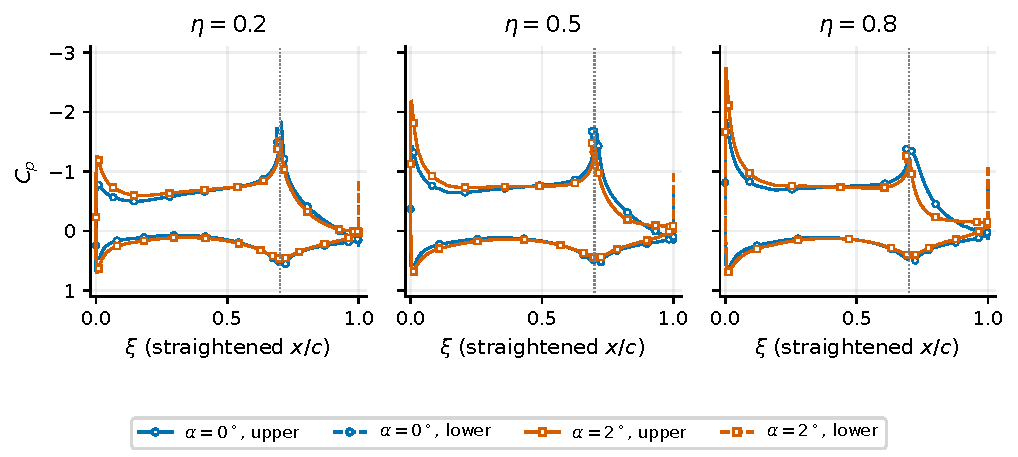
\includegraphics[width=\textwidth]{pressure_sections.pdf}
\caption{Connected numerical pressure sections for I/$\Gamma=0\degc$/$\delta=20\degc$ at direct $\alpha=0,2\degc$ and $\eta=s/b=0.2,0.5,0.8$. Circles: $\alpha=0\degc$; squares: $\alpha=2\degc$; solid: upper; dashed: lower. Each line segment follows an actual contour edge on a native fixed/control panel; junction, tip, and blunt-edge faces are excluded from these curves. The dashed vertical reference marks the 70\%-chord hinge. $\xi$ is the inverse-rotated local chord coordinate, not global $x/\bar c$.}\label{fig:cp}\end{figure}

The complete spatial integration in Fig.~\ref{fig:spatial} makes this pressure pattern quantitative. Over $\xi<0.4$, $0.4\leq\xi<0.7$, and $\xi\geq0.7$, ordinary lift increments are $+0.06706$, $-0.00966$, and $-0.03321$, whereas departures are $-0.03565$, $-0.03541$, and $-0.03955$. Both fixed-chord bins fall below their pre-feature trends. Thus stronger ordinary leading-edge suction does not establish unchanged fixed-surface effectiveness. The intermediate-chord loss and the reduced expected growth of the forward contribution both matter.

Geometric fore/aft lift increments, $+0.05740/-0.03321$, differ slightly from native fixed/control increments because junction allocation differs. This is a difference in region definitions, rather than a rescaling to close the budget. Pressure supplies almost all the principal lift departure (pressure $D_L=-0.11051$ versus total $-0.11060$); the small shear contribution is retained for accounting without a separate physical mechanism claim.

\begin{figure}[htbp]\centering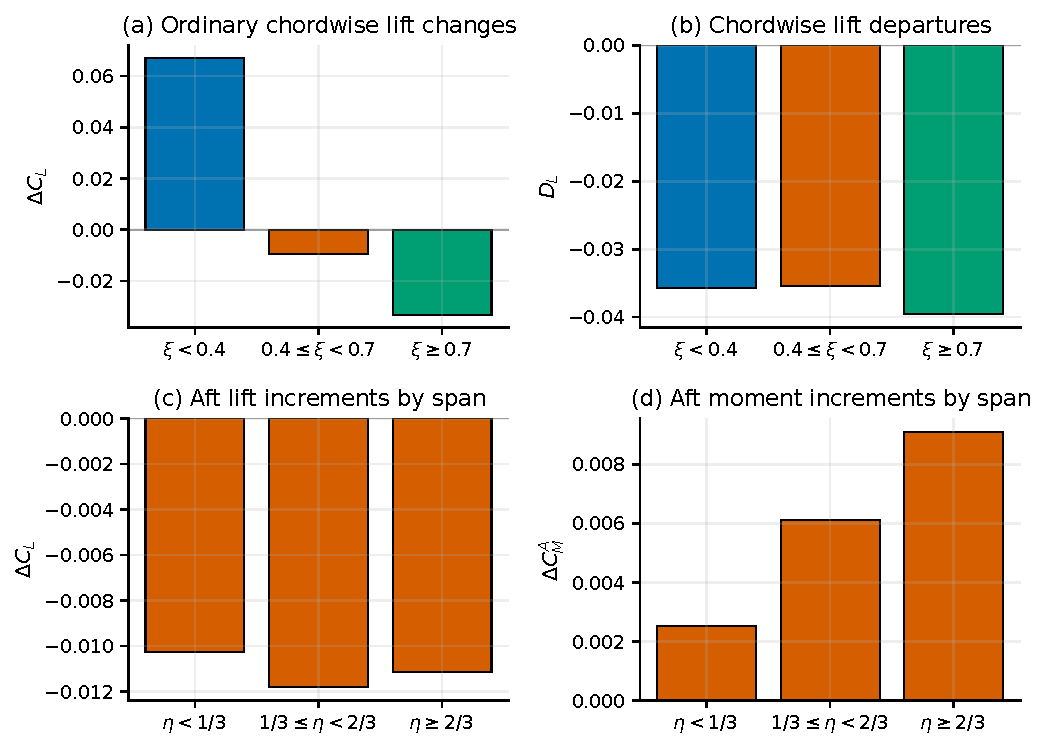
\includegraphics[width=\textwidth]{spatial_changes.pdf}
\caption{Integrated geometric-bin changes for I/$\Gamma=0\degc$/$\delta=20\degc$, direct $0\to2\degc$: (a,b) complete chordwise lift increments/departures, summed over span; (c,d) ordinary aft lift and moment increments over span thirds. Moment uses $x_A=0.642000000830$~m. Baseline is $\{-6,-4,-2\}\degc$. Both sides are included; endcaps remain separate in the complete totals. Bars are integrated dimensionless contributions, not coefficient densities or native marker groups.}\label{fig:spatial}\end{figure}

The aft span thirds lose similar ordinary lift, approximately $-0.01026,-0.01182,-0.01113$, yet their fitted-center moment increments rise from $+0.00252$ inboard to $+0.00612$ centrally and $+0.00910$ outboard. Similar force changes therefore produce different moment contributions through spatial weighting. About the original numerical origin, these same moment increments are $+0.00822,+0.01294,+0.01559$; the reference changes their magnitudes while the outboard weighting remains apparent. Shifting the inboard partition boundary from $1/3$ to $1/4$ changes the attributed regional share, while the whole-fore/whole-aft sums remain unchanged. Regional percentages are definition-dependent; their complete-domain sums and chordwise signs are the stronger result.

\subsection{Deflection contrast and reversal evolution}\label{sec:reversal}
The early I/$\delta=30\degc$ interval in Table~\ref{tab:budget} also combines a positive ordinary fixed lift increment with negative fixed and control departures. Its fitted-center moment contributions compete, and the total departure changes sign across windows, from approximately $-0.02616$ to $+0.00760$. A common sharply defined lift/moment event or a universal compensation mechanism cannot be imposed on both deflections.

Figure~\ref{fig:reversal} quantifies the accompanying numerical chordwise reversal. At I/$\delta=20\degc$, the upper-aft fraction grows from 0.1458 to 0.4850 over direct $0\to2\degc$; $\epsilon=10^{-5}$ gives 0.1450 to 0.4804. Reversal is already present at $-2\degc$ (0.1726), so this interval describes expansion, rather than first separation. At $\delta=30\degc$, the early fraction grows from 0.6216 to 0.9354 over $-10\to-8\degc$, with substantial reversal already present at earlier incidences. Reduced aft loading and a changed pressure distribution coexist with that expansion; ``pressure recovery'' here refers specifically to the chordwise rise in surface pressure downstream of the hinge suction minimum, without an inference that the boundary layer remains attached.

\begin{figure}[htbp]\centering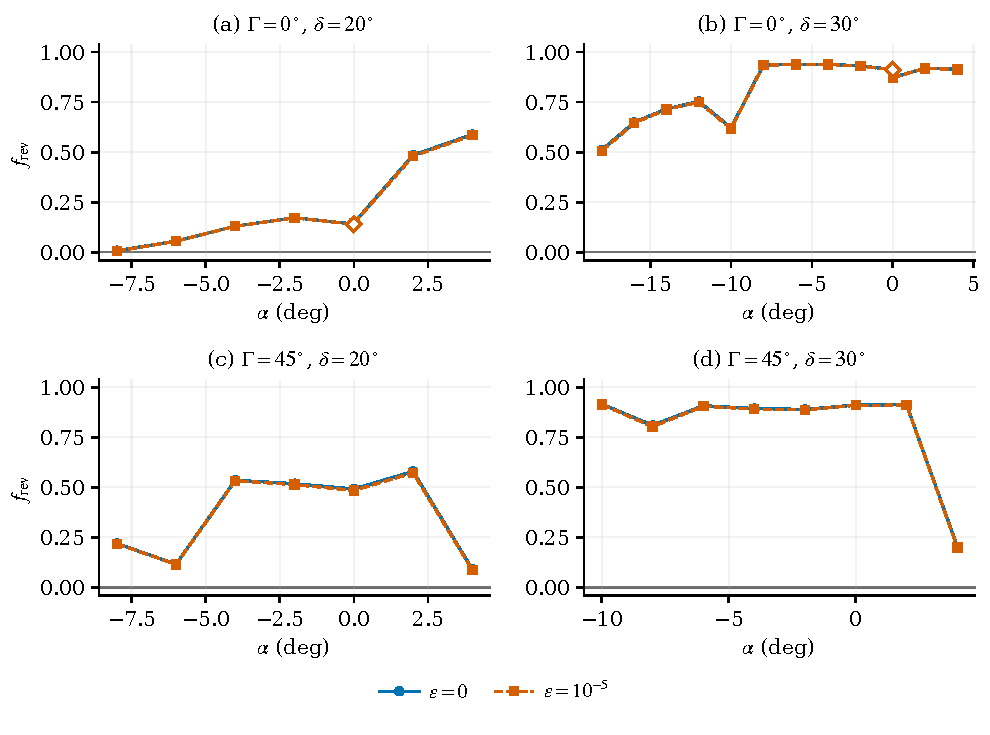
\includegraphics[width=\textwidth]{reversal.pdf}
\caption{Upper geometric-aft chordwise reversal fractions for Geom.~I at both dihedral settings and $\delta=20,30\degc$. Actual triangle area supplies the denominator. Circles/solid lines: $\epsilon=0$; squares/dashed lines: $10^{-5}$. Open diamonds distinguish reflected zero parents. Samples at $\alpha=4\degc$ are retained, including nonmonotonic dihedral behavior. The indicator measures reversed chordwise wall shear, not complete three-dimensional separation area.}\label{fig:reversal}\end{figure}

For I/$\Gamma=45\degc$/$\delta=30\degc$, the control is already extensively reversed around the selected moment interval: 0.8890 to 0.9108 over $-2\to0\degc$. Later inclined samples are nonmonotonic: $\delta=20\degc$ falls from 0.5790 at $2\degc$ to 0.0900 at $4\degc$, and $\delta=30\degc$ from 0.9124 to 0.2031. These saved-state changes are not smoothed away or assigned a reattachment cause or hysteresis.

For the specific inclined $\delta=30\degc$, $\alpha=2\degc$ case, wall output in the upper outboard leading-edge region ($2/3\leq\eta\leq0.95$, $0\leq\xi\leq0.15$) contains reversing chordwise shear and low modeled BCM intermittency. On the reversing-centroid subset, median intermittency is approximately $2.4\times10^{-5}$ and maximum $8.6\times10^{-5}$. Wall eddy viscosity and SA working variable are zero there. These wall quantities indicate the local model setting, but do not identify a boundary-layer profile or prove a laminar separation bubble. That classification is not used.
\FloatBarrier

\section{Dihedral and Planform Dependence}\label{sec:geometry_effects}
\subsection{Matched dihedral: levels and incidence changes}\label{sec:dihedral}
The dihedral comparison holds Geom.~I, $\delta$, $\alpha$, $S$, and MAC fixed. Orientation and the associated root cut/domain change together. The two settings support a controlled comparison within this dataset, without interpolation to smaller dihedral angles or generalization to aircraft tails.

Measured $\delta=20\degc$ primary lift departures over $-2\to0\degc$ are $-0.08274$ at zero dihedral and $-0.04785$ at $45\degc$. Relative to each fitted preceding increment, the descriptive deficits are 80.6\% and 76.4\%. Over $-2\to2\degc$, they become 64.5\% and 82.2\%. Smaller absolute deficits with dihedral therefore do not imply universally smaller relative suppression. These interval-dependent ratios have no assigned significance level.

Absolute numerical load projection supplies context for this distinction. At $\alpha=0\degc$, $\delta=20\degc$, the matched lift difference is $C_{L,45}-C_{L,0}=-0.30147$. In a local span/normal coordinate decomposition, projection of the zero-dihedral normal loading contributes $-0.24666$, changed local normal loading $-0.04898$, and local span-force projection $-0.00582$; the axial term is zero at this incidence. This is algebraic coordinate accounting of a level difference, rather than a causal isolation of dihedral-induced separation or an explanation of nonlinear growth suppression.

For the incidence-dependent moment comparison, Fig.~\ref{fig:dihedral} instead evaluates
\begin{equation}
 \mathcal I_M=[C_{M,45}^{A_I}(\alpha_b)-C_{M,45}^{A_I}(\alpha_a)]
             -[C_{M,0}^{A_I}(\alpha_b)-C_{M,0}^{A_I}(\alpha_a)]
\label{eq:interval}
\end{equation}
with the same intervals and physical numerical axis. The corresponding $z\,dF_x$ and $-(x-x_{A_I})dF_z$ terms complete its sum. For $\delta=30\degc$ over $-2\to0\degc$, $\mathcal I_M=-0.01836$, split into $-0.00808$ and $-0.01027$. Both terms contribute to the change in moment response with dihedral. This is an ordinary interval contrast, without baseline subtraction. It connects geometric moment weighting to incidence-dependent loading without presenting moment translation itself as a new mechanism.

\begin{figure}[htbp]\centering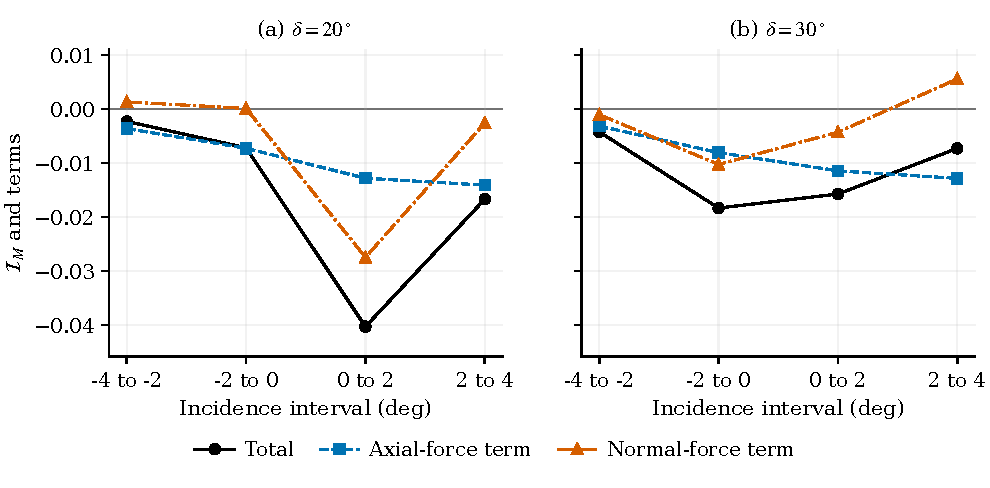
\includegraphics[width=\textwidth]{dihedral_intervals.pdf}
\caption{Matched Geom.~I dihedral contrasts of ordinary moment increments, $\Gamma=45\degc$ minus $0\degc$, at identical $\delta=20\degc$ (left) and $30\degc$ (right). All moments use the common axis $A_I=(0.642000000830,0,0)$~m. Contributions are the integrated terms in Eq.~\ref{eq:moment}; their sum is the total in Eq.~\ref{eq:interval}. Direct zero parents are used; there is no empirical baseline subtraction in this figure.}\label{fig:dihedral}\end{figure}

\subsection{Second planform and scope of the result}\label{sec:planform}
For II/$\delta=20\degc$, Table~\ref{tab:budget} shows positive ordinary fixed-surface lift growth and negative control growth. Both lift departures are negative. At its retained fitted center, however, both moment departures are positive: $+0.00751$ fixed and $+0.00710$ control, with total $+0.01461$. Thus the available fitted-center budget supports reinforcement, rather than fixed/control cancellation. Partial cancellation about the original numerical origin is a different result: fixed $-0.00231$, control $+0.00352$, and total $+0.00121$. That small total is baseline- and zero-parent-sensitive, and does not explain the experimental fitted-center feature.

The reflected Geom.~II zero parent gives a lift increment $+0.11209$ rather than $+0.09351$ on $0\to2\degc$ and fitted-center moment departure $+0.00698$ rather than $+0.01461$. Each force and field pair remains state-consistent. These alternate numerical states are not evidence of a hysteresis experiment. The measured lift slowdown remains poorly reproduced, despite a locally similar direct-state moment increment. Moreover, $\lambda$, $\tau$, $\Lambda$, chord distribution, area, and MAC Reynolds number all differ from Geom.~I. No isolated negative-sweep law follows.

The engineering information supplied by these results is a distinction between total-load growth and control/load effectiveness: a positive integrated increment can conceal a substantial deficit in both fixed and deflected contributions. Moment additionally weights where those changes occur, so a lift-only or constant-derivative description loses information about load allocation and reference-specific pitching response. The existing dataset supports these quantified comparisons for its tested geometry and conditions. It does not determine how an unswept wing, greater sweep, a partial-span control, another flap chord, or another taper alone would change the response, and it does not establish general lower-order prediction failure.
\FloatBarrier

\section{Conclusions}\label{sec:conclusions}
The existing MONNALISA data support a quantitative extension from known control-surface separation to joint fixed/control loading response. LE1 measurements establish sampled lift-growth changes and separately signed moment changes; weak inclined moment features and the curved early $30\degc$ sequence require uncertainty and interval qualifications. A universal joint $20\degc$ threshold and a common precise lift/moment onset are unsupported.

In the baseline I/$\Gamma=0\degc$/$\delta=20\degc$ numerical interval, ordinary fixed-surface lift growth coexists with a substantial deficit from its preceding trend. Both fixed and control contributions fall below that trend, with about 63\% of the total lift departure allocated to the fixed part across the tested definitions. Sectional pressures and full spatial budgets show forward ordinary suction growth alongside hinge/aft losses; both fixed-chord bins contribute to reduced expected growth. The fitted-center moment departures reinforce, with a different component ranking from lift and different spanwise weighting of similar aft force losses.

Matched dihedral results distinguish lower absolute lift from relative suppression and show material changes in both moment-arm terms across incidence. The second planform also has reinforcing fitted-center moment departures; its response cannot be interpreted as an isolated sweep effect. Reversal expansion accompanies the numerical loading changes but predates some integrated features and is not the new contribution by itself.

The principal limitation is partial WT--RANS correspondence, including baseline lift bias, inclined numerical irregularities, and an inadequately reproduced Geom.~II lift slowdown. Existing mesh evidence supports integrated-load sensitivity only at the published $35\degc$ conditions. The detailed joint and spatial loading results describe the computed states, rather than an experimentally validated universal separation mechanism.
\FloatBarrier

\appendix
\section{Sensitivity of the Numerical Loading Interpretation}\label{app:sensitivity}
Table~\ref{tab:sensitivity} keeps the absolute baseline departure and its allocation separate. The three unweighted windows use the same samples for all components. Direct and reflected zero parents are not averaged. The earliest pre-feature window has appreciable curvature; the positive fitted-center moment departure and fixed lift fraction persist even though the total lift deficit varies.

\begin{table}[htbp]\centering\small
\caption{I/$\Gamma=0\degc$/$\delta=20\degc$, $0\to2\degc$: baseline and zero-parent sensitivity. $D_M^A$ uses $x_A=0.642000000830$~m. Fixed fraction is $D_{L,\mathrm{fixed}}/D_{L,\mathrm{total}}$, without an assigned confidence level.}\label{tab:sensitivity}
\begin{tabular}{llrrr}\toprule
Zero parent & Baseline (deg) & Total $D_L$ & Fixed fraction (\%) & Total $D_M^A$ \\\midrule
Direct & $\{-6,-4,-2\}$ & -0.110605 & 62.55 & +0.033238 \\
Direct & $\{-8,-6,-4\}$ & -0.136788 & 62.43 & +0.040913 \\
Direct & $\{-4,-2,0\}$ & -0.105014 & 62.64 & +0.033958 \\
Reflected & $\{-6,-4,-2\}$ & -0.111790 & 62.76 & +0.033493 \\
Reflected & $\{-8,-6,-4\}$ & -0.137973 & 62.60 & +0.041168 \\
Reflected & $\{-4,-2,0\}$ & -0.106792 & 62.98 & +0.034341 \\

\bottomrule\end{tabular}\end{table}

The whole fore/aft sums survive the tested span-third versus span-quarter partition; finer chord bins preserve the two negative fixed-chord departures. Redefining the inboard aft boundary from $\eta<1/3$ to $\eta<1/4$ changes its lift departure from $-0.01270$ to $-0.00939$. This is partition sensitivity, not a regional discretization-error estimate. Exact native-marker matching is available for six direct baseline states, with complete facet coverage; other spatial results use geometric bins explicitly.

The I/$\delta=20\degc$ upper-aft reversal fraction at direct zero is 0.14578 versus 0.14089 at the reflected zero. Threshold $10^{-5}$ changes the direct $0\to2\degc$ sequence to 0.14497--0.48043, preserving growth. Typical stored vector skin-friction norms are of order $10^{-3}$; the small thresholds test near-zero sensitivity, without a statistical uncertainty interpretation.

At the original numerical origin, the baseline total moment departure is $+0.10028$, with fixed $+0.05286$ and control $+0.04743$. At the retained fitted center the total is $+0.03324$, fixed $+0.01069$, and control $+0.02255$. This reference dependence changes allocation while retaining reinforcement. All reference transports use body $C_{F,z}$ in Eq.~\ref{eq:transport}, rather than lift. The principal experimental comparison remains at its own fitted center and is not reassigned to either numerical axis.
\FloatBarrier
\section*{Acknowledgments}
This project has received funding from the Clean Sky 2 Joint Undertaking (JU) under grant agreement No 101008257. The JU receives support from the European Union's Horizon 2020 research and innovation programme and the Clean Sky 2 JU members other than the Union.
\bibliography{References}
\end{document}
